\chapter{语音转换系统}

\section{概述}

如前文所述,语音转换是一种在保持语音中文本内容不变的前提下,将语音中的说话人信息转变为另一说话人信息的技术。
目标说话人可以是特定说话人,也可以是非特定的。本文将主要讨论特定说话人的语音转换。

\begin{figure}[!htp]
    \centering
    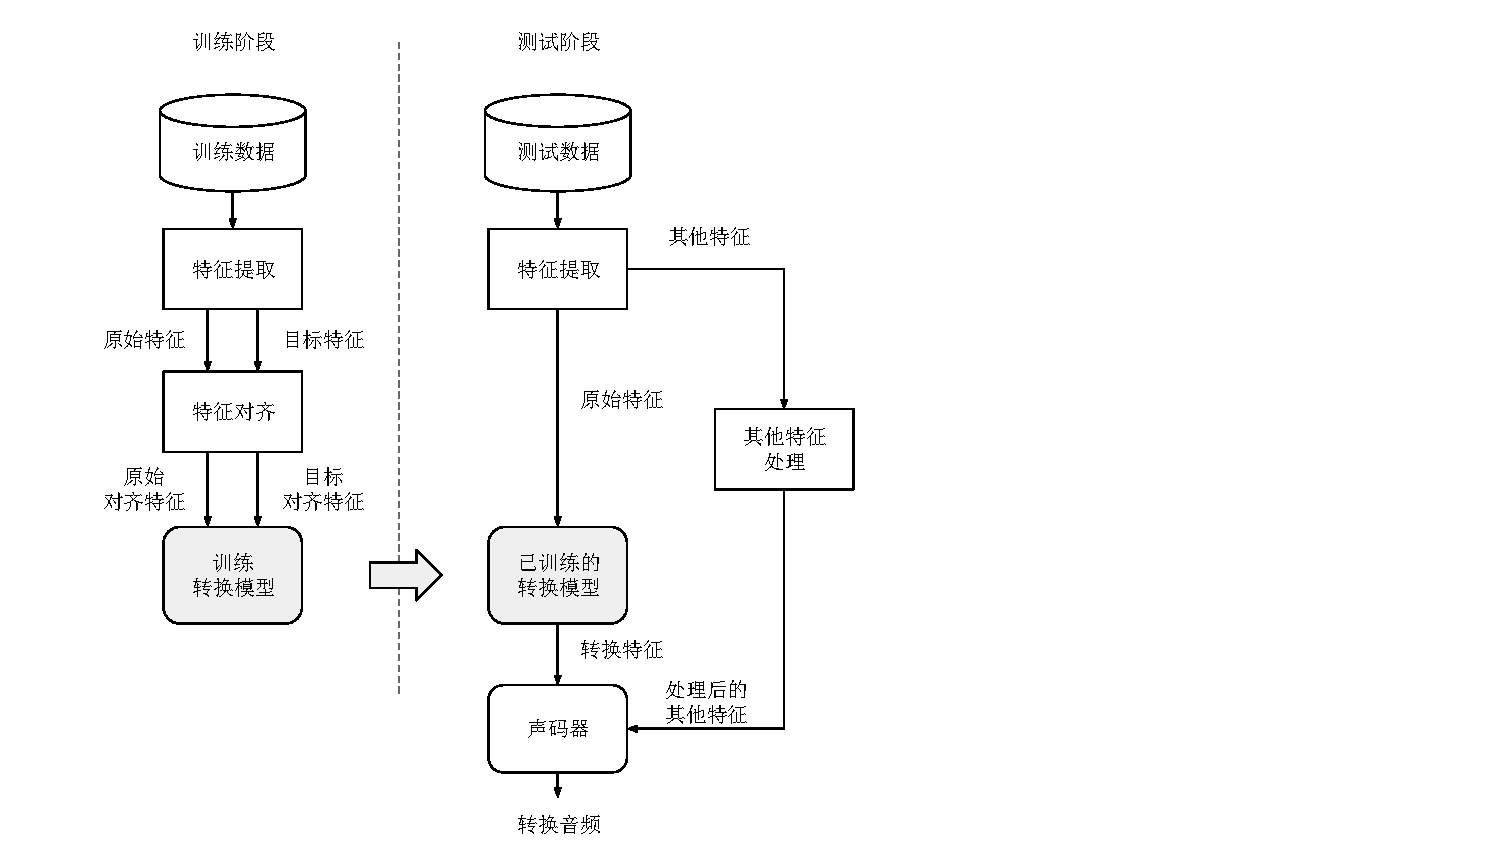
\includegraphics[width=8cm,trim=50 0 310 10,clip]{figure/2_vc_basis.pdf}
    \bicaption[语音转换系统示意图]
    {语音转换系统示意图}
    {Schematic diagram of the voice conversion system}
    \label{fig:vc_basis}
\end{figure}

如图~\ref{fig:vc_basis}所示,语音转换系统通常包含训练模块和测试模块。在训练阶段,首先需要从训练数据中
提取声学特征,通常使用传统的数字信号声码器实现该部分;之后将提取出的原始和目标声学特征进行对齐,对齐算法
取决于使用的语音转换方法,有些转换方法也会省略掉对齐步骤;对齐后的特征会放入转换模型中根据具体的方法进行训练。在测试阶段,测试数据中只有
原始说话人的数据,首先用声码器提取声学特征;然后将特征输入已经训练完成的转换模型中得到转换特征;通常声码器
分析出的特征不只一种,有些方法只会转换一部分声学特征,剩下的其他特征需要做其他处理,如线性变换,保持不变等;
最后将处理后长度相等的声学特征放入声码器中,得到转换音频。

可以看出,决定语音转换系统性能的主要因素为语音分析和合成方法,特征对齐和转换模型。目前的神经网络声码器已经可以稳定地从
真实音频分析的特征中生成非常自然的声音了,因此只要转换模型转换出来的特征足够接近真实,那么声码器就可以等价地生成接近真实的语音。
特征对齐对语音转换的性能有着较大的影响,对于序列层面的对齐而言,受到说话人语速、韵律的影响,长度不同的两段特征往往很难做到精准的对齐,
错误的对齐则会导致向训练数据数据引入错误的标签。因此,近两年提出了很多绕开特征对齐的语音转换方法。转换模型是语音转换中非常重要
的一步,除了能够进可能地转换说话人信息之外,现有的转换模型大多只考虑对说话人信息进行转换,对于韵律特征(如基频,时长)则依旧采用简单的线性变换,
这种变换可以得到不错的效果,但很难真实反应目标说话人的韵律变化,因此较为复杂的韵律转换方法也成为语音转换的目标之一。

评价一个语音转换系统的好坏主要根据该系统所转换的语音来判断,一般分为客观指标和主观指标。
客观指标一般采用梅尔倒谱失真(Mel-cepstral Distortion,MCD)或对数谱失真(Log-Spectral Distortion, LSD),
梅尔倒谱失真计算方法如下,

$$MCD(a^{cvt}, a^{tgt})=\frac{10\sqrt{2}}{ln10T}\sum^{T-1}_{t=0}\sqrt{\sum^{D}_{d=s}(a^{cvt}_{d}(t)-a^{tgt}_{d}(t))^2}$$

其中$a^{cvt}$和$a^{tgt}$分别代表转换特征序列和目标特征序列,$T$和$D$分别代表时间维度和特征维度的大小。梅尔倒谱失真
的计算方法也可以应用到其他特征的失真计算中,如梅尔频谱失真,失真度越小,系统的性能就越好。客观指标可以一定程度上反应转换特征和真实特征之间的差异程度,
但由于语音的质量通常由很多复杂的因素决定,客观指标的计算往往不能充分反应音质的好坏。对于语音生成任务而言,
语音的最终接收者是人,因此最能反应生成语音好坏的方法就是主观评价。主观评价测试可以分为主观意见分测试(Mean Opinion Score, MOS)和对比测试(ABX test)。
主观评价测试一般由测试人员对音频做出1到5分的打分,相似度则需要测试人员在候选音频中选择自己更为偏好的一个。
通过若干名客观的测试人员对测试音频的两个方面进行打分,分别为自然度和相似度。自然度表示语音是否像是人类发出的声音,具体
体现在语音的连贯性,噪音以及音调上。相似度表示语音中的说话人是否像是目标说话人的声音,具体体现在语音的音色上,韵律对相似度也有一定的影响。


\section{语音分析和合成方法}
音频的数字形式可以看成一段长度较长的实数序列,序列的长度由音频时长和采样率决定。例如对于16k采样率的一秒时长的音频,
则可以表示为一个长度为16000的向量,直接对音频样本点序列进行建模目前还有比较大的难度。因此通常会基于语音的短时平稳的特性,
对样本点序列进行分窗成帧,由于每一窗内的信号可以认为是平稳的,则可以对窗内的信号进行分析提取特征,这样可以大大缩短音频表示的序列长度。
因此作为语音转换的主要对象,声学特征的分析对转换模型的建模复杂度和声码器的合成音质都有非常直接的影响。常见的声学特征及其特性如表~\ref{tab:vc_feats}所示\cite{Nurminen2012Voice}。

\begin{table}[!hpt]
    \bicaption{常用语音转换声学特征示例}{Typical acoustic features used in voice conversion}
    \label{tab:vc_feats}
    \centering
    \begin{tabular}{p{0.3\columnwidth}p{0.6\columnwidth}} 
        \toprule
        声学特征 & 注释 \\
        \midrule
        线谱信号频率(LSF) & 提供稳定,良好的插值性;与共振峰相关性强;对频谱峰建模 \\
        梅尔频率倒谱系数(MFCCs) & 对频谱峰和频谱谷建模;由于对声学距离度量的可靠性,对特征对齐十分有用 \\
        梅尔倒谱系数(MCCs) & 是语音转换和基于HMM的语音合成技术中最常用的频谱表示特征之一。在特征对齐上和MFCCs类似 \\
        共振峰(Formants) & 共振峰的带宽,位置和强度将会是语音转换中非常有用的特征,但是它们的有效估计仍具有挑战性 \\
        频谱采样点 & 频域的采样点也可以被用作语音转换的特征;一般多用于基于频率弯折的方法中。\\
        \midrule
        基频($F_0$) & 基频和对数基频一般通过均值方差的变换转换到目标说话人 \\
        \midrule
        发音标志(Voicing) & 通常二值的发音或非周期信息 \\
        \midrule
        激励频谱 & 有时激励频谱的细节也需要被建模,一般在使用正弦模型是会被用到。\\
        \bottomrule
    \end{tabular}
\end{table}

对于语音的合成方法,可以通过数字信号声码器和神经网络声码器来实现。数字信号声码器通过信号处理的手段
从特征合成音频,主要包括STRAIGHT声码器,WORLD声码器和GL算法;神经网络声码器则是通过神经网络
从大量音频数据中学习特征与音频样本点之间的关系,包括WaveNet, WaveRNN, LPCNet等。
下文将详细介绍源滤波器模型和几种常用的数字信号声码器和神经网络声码器。

\subsection{源滤波器模型}
源滤波器模型是发声理论中非常著名的模型。在源滤波器模型看来,人类的发声过程主要由声道系统完成,
可以分为两个阶段:激励和滤波。其中源激励由喉中的声带产生,滤波由声道的谐振特性完成。
对于元音而言,声源是由声带周期性震动产生的一定频率的声门声音,声源决定元音的音调和音质,
之后由声道和口腔的谐振特性对输入声源进行滤波,得到了不同的元音发音。对于辅音而言,声源主要由
气流在声带,咽部等经过时发出的非周期信号组成,滤波部分同元音类似。声源并不是单一的,实际产生
的声音中往往包含一个或多个声源。发声是一个动态的过程,当声道配置出现改变时,
其谐振特性也会出现改变,随之改变音质和输出的声音。

\begin{figure}[!htp]
    \centering
    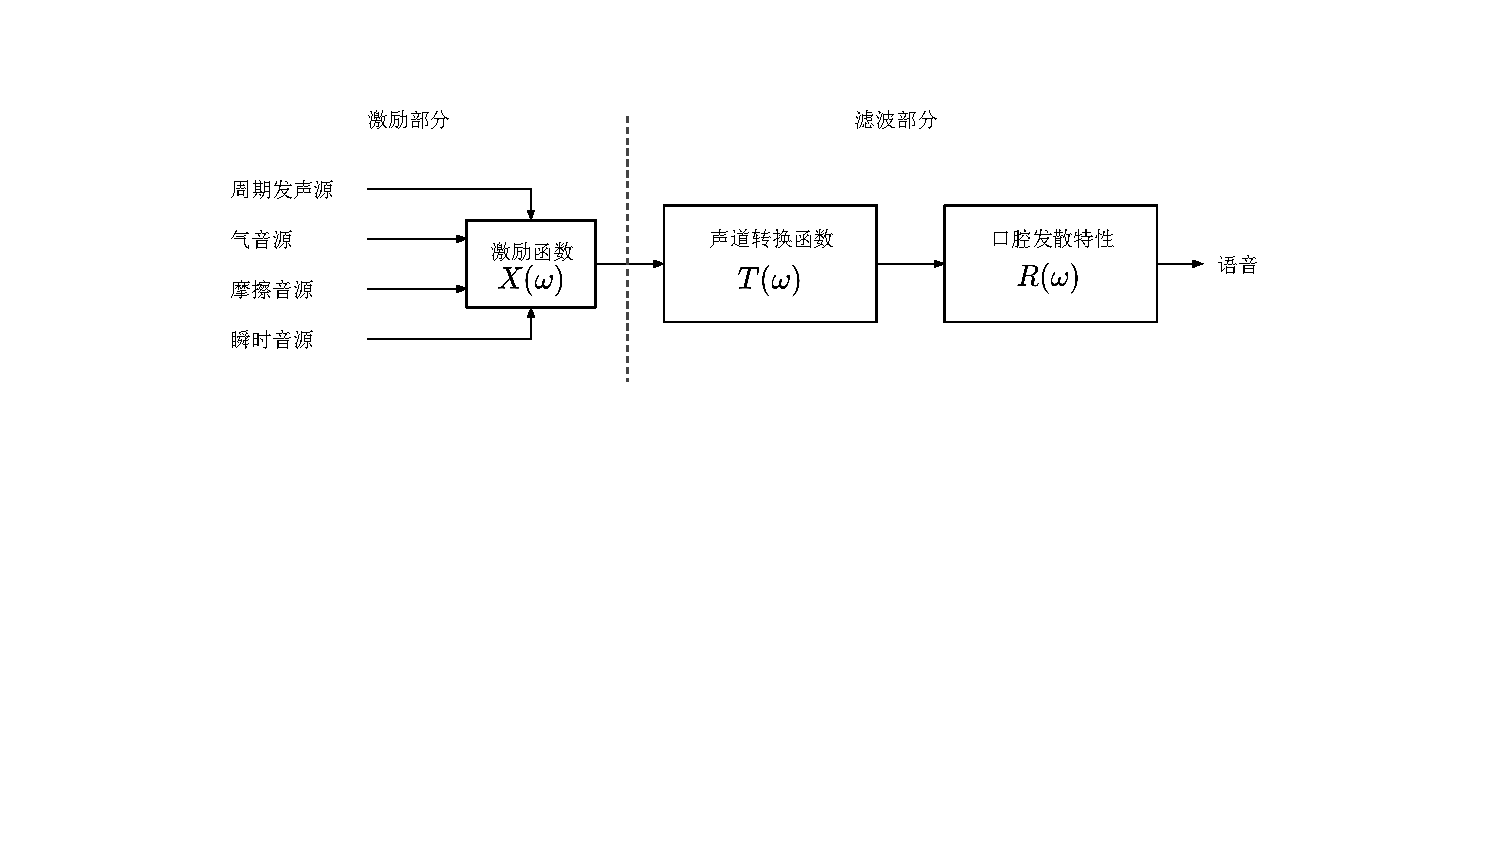
\includegraphics[width=13cm,trim=100 210 100 40,clip]{figure/2_sourcefilter.pdf}
    \bicaption[源滤波器模型示意图]
    {源滤波器模型示意图}
    {Schematic diagram of the source filter model}
    \label{fig:sourcefilter}
\end{figure}

图~\ref{fig:sourcefilter}是源滤波器模型的示意图。不管是元音还是辅音,都会涉及到四种声源:声门周期震动时产生的带有基频的发声源,当空气快速通过
开放不震动的声门时产生的气音源,当空气快速通过狭窄的咽部时摩擦产生的摩擦音源,口腔中压力突然改变而
产生的瞬时音源。其中发声源属于周期信号源,气音源、摩擦音源和瞬时音源属于非周期信号源。
当人类产生声音时,一种或多种音源的组合会作为输入传递给声道滤波,所发出的元音或辅音则可以看做
滤波的输出。

如果声道的配置不发生改变,声道滤波部分就会变成一个线性时不变系统(LTI),同时输出信号$y(t)$
可以由输入信号$x(t)$和系统的冲激响应$h(t)$的卷积来表示,也就是
\begin{equation}
    y(t) = h(t) * x(t)
\end{equation}
转换成频域表达就是
\begin{equation}
    Y(\omega) = H(\omega) X(\omega)
\end{equation}
也就是说,语音谱$Y(\omega)$是由源谱$X(\omega)$和声道滤波谱$H(\omega)$的乘积建模而成。
严格来讲,声道滤波谱$H(\omega)$可以被进一步拆分为声道转换函数$T(\omega)$和口腔的发散特性$R(\omega)$
的乘积,即
\begin{equation}
    Y(\omega) = [T(\omega)R(\omega)]X(\omega)
\end{equation}

源滤波器模型对声音的产生给出了很好的解释和模拟,但也存在较多缺陷。一方面是声源信号的实际处理过程涉及
到更多复杂的非线性变换,直接的线性操作很难模拟真实语音,同时语音的产生是一个时变的过程,声道的配置
根据实际情况不断变化,这些变化的建模也是语音发声的难点之一。但由于源滤波器模型的有效性,其仍受到了
广泛的使用。


\subsection{数字信号声码器}
数字信号声码器是指利用信号处理技术对音频进行特征分析和重建的一系列技术。由于其通常包含了从语音提取特征和
从特征合成语音的一系列功能,从而是语音转换和语音合成等语音生成任务中使用最广泛的一类声码器。接下来将介绍
常用的两个数字信号声码器:STRAIGHT,WORLD,Griffin Lim。

\begin{itemize}
    \item \textbf{STRAIGHT:}全称为自适应内插加权谱的语音转换与重构模型(Speech Transformation
    and Representation using Adaptive Interpolation of weiGHTed spectrum),于1997年提出\cite{kawahara1997speech}。

    \begin{figure}[!htp]
        \centering
        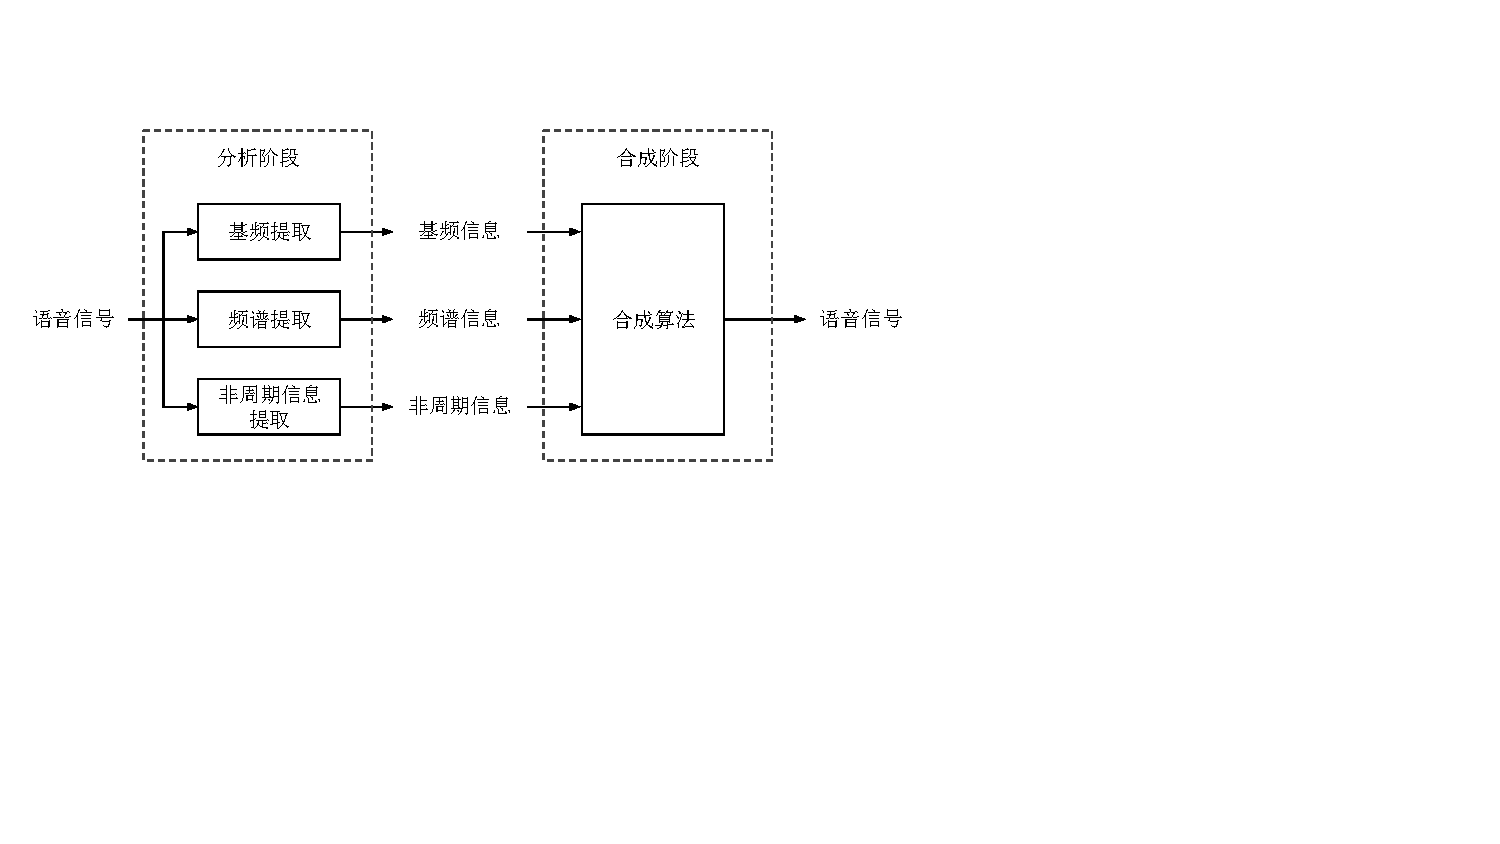
\includegraphics[width=13cm,trim=10 180 280 60,clip]{figure/2_vocoder.pdf}
        \bicaption[STRAIGHT声码器模型框架]
        {STRAIGHT声码器模型框架}
        {Framework of the STRAIGHT vocoder}
        \label{fig:vocoder}
    \end{figure}

    STRAIGHT建立在源滤波器理论上。如图~\ref{fig:vocoder}所示,STRAIGHT通过语音分析从语音信号中提取出三个独立性较强的特征:基频,幅度谱和
    非周期信息。其中基频代表上文中激励部分的频率,也代表语音中的音调高低频率;幅度谱代表语音的在各个频率
    上的福值,可以看成滤波部分中的滤波器分量,决定语音的发音;非周期信息则描述了周期信号和非周期信号之间
    的比例关系,对语音的自然度有很大的作用。STRAIGHT在传统源滤波器信道声码器(VOCODER)的基础上,通过
    在时频域对功率谱进行谱补偿的平滑处理,并在时间轴和频率轴上采样,消除自然语音中周期性的方法来提高语
    谱估计的准确度,进而提升重构语音的音质\cite{杨骋基于简化}。STRAIGHT是传统语音生成任务中最常用的声码器之一。
    \item \textbf{WORLD:}WORLD于2016年作为能够实现高质量实时合成的声码器被提出,由于其在不降低音质的
    情况下高效的合成速度和免费开源的特性,很快就吸引了大量研究者的使用\cite{morise2016world}。与STRAIGHT类似,WORLD也是基于
    源滤波器模型。在WORLD中,首先基频轨迹使用DIO基频提取算法从音频中估计;然后用CheapTrick算法分析频谱,
    分析频谱时不光需要原始音频,也需要上一步提取的基频;最后用PLATINUM算法从原始音频、基频和频谱中估计
    非周期信息。其中WORLD中的非周期信息定义与STRAIGHT中略有不同,STRAIGHT中非周期信息是指非周期信号
    与周期信号之间的比例,而WORLD中则是直接将激励信号作为非周期信息。在合成部分,声带振动是在最小相位
    响应的卷积基和提取的激励信号上计算的,相比STRAIGHT,卷积计算量更小,使得合成速度也会更快。
    \item \textbf{Griffin Lim:}Griffin Lim(GL)于1984年作为一种信号重建算法被提出\cite{griffin1984signal}。
    它可以实现从信号的短时傅里叶变换中估计信号。GL算法的优点是可以直接从频谱构建音频,而不需要预先知道
    相位信息,相位信息由算法估计。缺点是相位的估计依旧不够精准,合成的声音依旧有较为明显的相位不准的情况。
    GL算法首先初始化相位,然后通过不断的计算逆傅里叶变换和傅里叶变换来估计相位信息,一般50次迭代就可以得到
    效果不错的音频。但由于算法本质上是一种迭代算法,因此很难做到实时。
\end{itemize}

目前的数字信号声码器在语音合成的鲁棒性和特征可修改性上都有较好的表现,如STRAIGHT可以实现对音调、声道长度和语速等特性进行600\%
的修改而不会导致音质的明显下降。同时WORLD在处理速度和实时性上也有较好的表现。但当前数字信号声码器所存在的普遍问题
是合成音质与真实音频还有着较大的差距,主要体现在STRAIGHT和WORLD通常会有较为明显的蜂鸣声,由于基频预测不准确
造成的额外噪音,以及人声的不自然。这些一部分是因为数字信号声码器的实现主要是基于信号处理领域的先验知识,声码器和
现实生活中的真实语音并不存在信息交互,由于语音中实际存在大量的复杂信息,仅通过源滤波器模型来模拟语音生成过程是不足以良好的重建语音的。
因此基于深度学习的声码器逐渐被提出,其通过学习大量真实数据,使得语音合成的自然度有了飞跃性的提升。

\subsection{神经网络声码器}
神经网络声码器是指通过神经网络强大的非线性建模能力,来实现从声学特征到音频的合成技术。不同于数字信号声码器,
神经网络声码器通常需要大量的真实音频数据对合成模型进行训练。本文主要介绍两种神经网络声码器:WaveNet和LPCNet。

\begin{itemize}
    \item \textbf{WaveNet:}WaveNet于2016年由谷歌首次提出,最初是作为音频生成模型来实现自然音频的生成\cite{oord2016wavenet}。
    并将其在语音生成,文本转语音,音乐生成和语音识别任务上进行了初步尝试,并在2017年被成功应用到声码器上\cite{tamamori2017speaker}。
    
    \begin{figure}[!htp]
        \centering
        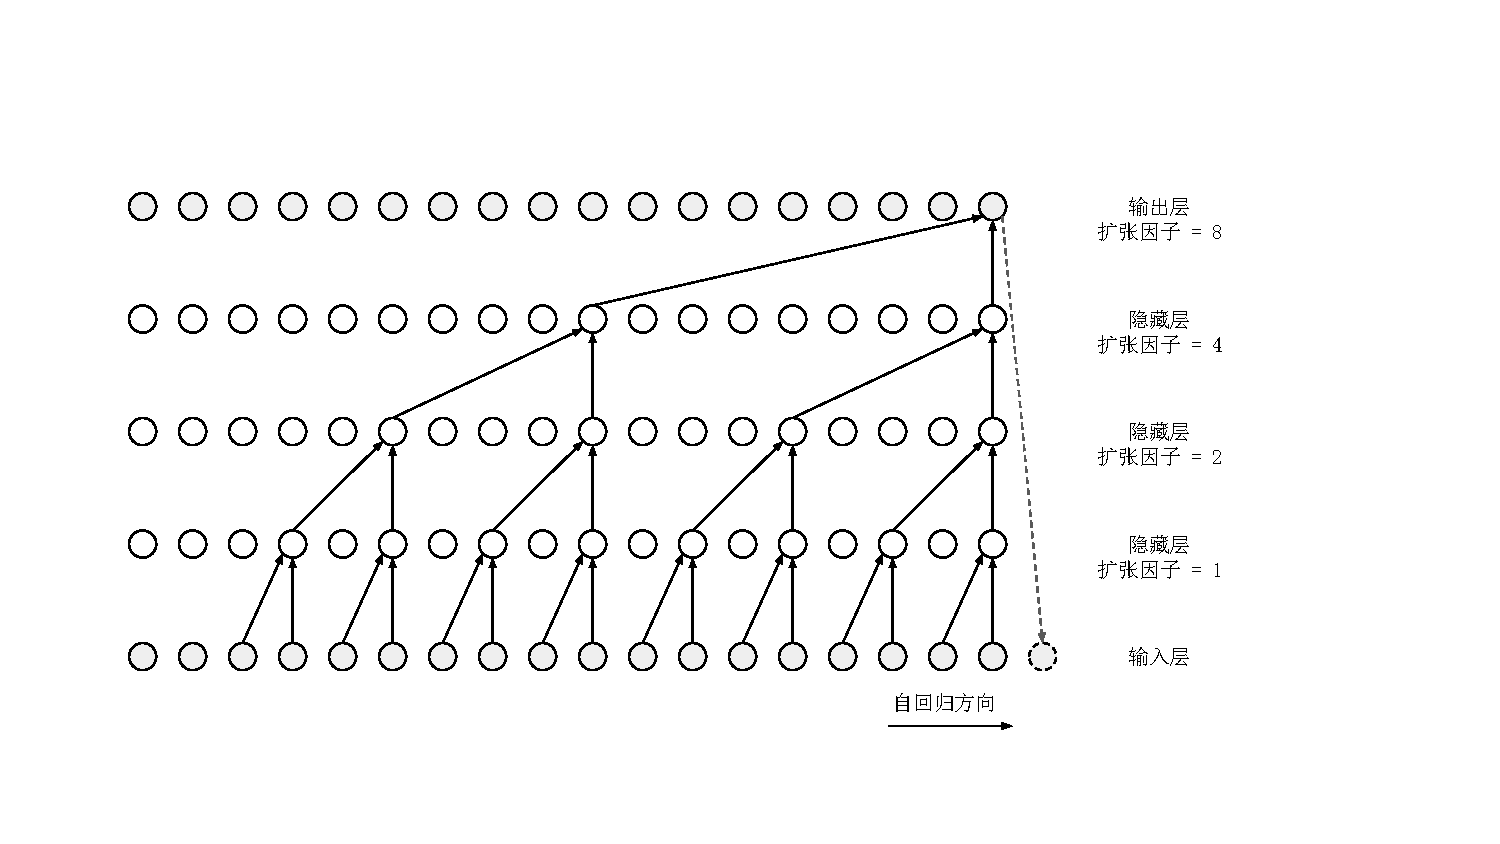
\includegraphics[width=13cm,trim=30 50 130 80,clip]{figure/2_wavenet.pdf}
        \bicaption[WaveNet自回归示意图]
        {WaveNet自回归示意图}
        {Schematic diagram of the autoregressive WaveNet}
        \label{fig:wavenet}
    \end{figure}

    如图~\ref{fig:wavenet}所示,WaveNet是一种自回归模型,即当前时刻的输出取决于之前历史的输出。
    每一个时刻模型会通过音频历史的样本点来预测当前的样本点。由于音频的样本点非常密集,一秒种的音频
    就有上万个样本点,这对自回归模型而言建模难度非常大,因此WaveNet提出使用扩张的因果卷积来增加
    模型的感受域。因果是指模型只会将历史样本点作为输入,预测当前样本点;扩张是指模型会在每层将相隔
    一定距离的样本点作为输入,而不是将所有样本点作为输入。例如图~\ref{fig:wavenet}中隐藏层从低到高
    扩张因子分别为1,2,4,8,即为2的n次方,这样可以使得每一层只有两个输入的情况下,只用4个隐层便
    达到16的感受域。

    WaveNet也可以通过在每一层添加额外的输入来实现在音频生成的过程中加入条件向量,该条件向量即可以是句子级别
    的,也可以是帧级别的,分别对应全局条件和局部条件。在WaveNet声码器中,条件向量可以是任何声学特征,全局
    向量可以代表说话人,实现多说话人的声码器。WaveNet可以生成非常接近自然的语音,但是其缺点也非常明显,
    WaveNet生成时间较长,很难实现实时生成,因此一些提升WaveNet生成效率的改进也被提出,如Parallel WaveNet\cite{oord2017parallel}。
    
    \item \textbf{LPCNet:}LPCNet于2019年提出,是一种高效且实时的神经网络声码器。
    其以WaveRNN声码器\cite{kalchbrenner2018efficient}为基础,结合了深度学习和数字信号处理,显式
    加入了线性预测系数(Linear Prediction Coefficients, LPC)来降低神经网络建模的复杂度。LPCNet可以
    分为两个子网络,帧级别网络和采样点级别网络,以及一个计算LPC的模块。在生成过程中,
    帧级别网络对输入的每一帧声学特征计算条件向量,LPC模块从声学特征中计算LPC,两个特征在帧内保持不变。
    采样点级别网络根据一帧对应的特征,以自回归的方式预测样本点。相比WaveNet, LPCNet的计算复杂度很低,
    可以高效地实现实时合成。
\end{itemize}

\section{特征对齐}
在实际情况中,两个不同的说话人说同一句话时时间长短往往是不一样的,因此就需要对两段对应的特征序列进行对齐操作,
将它们统一成相同的长度。由于特征对齐的情况大多在平行语料的语音转换中出现,因此本文主要说明平行语料语音转换中
的特征对齐。

\begin{figure}[!htp]
    \centering
    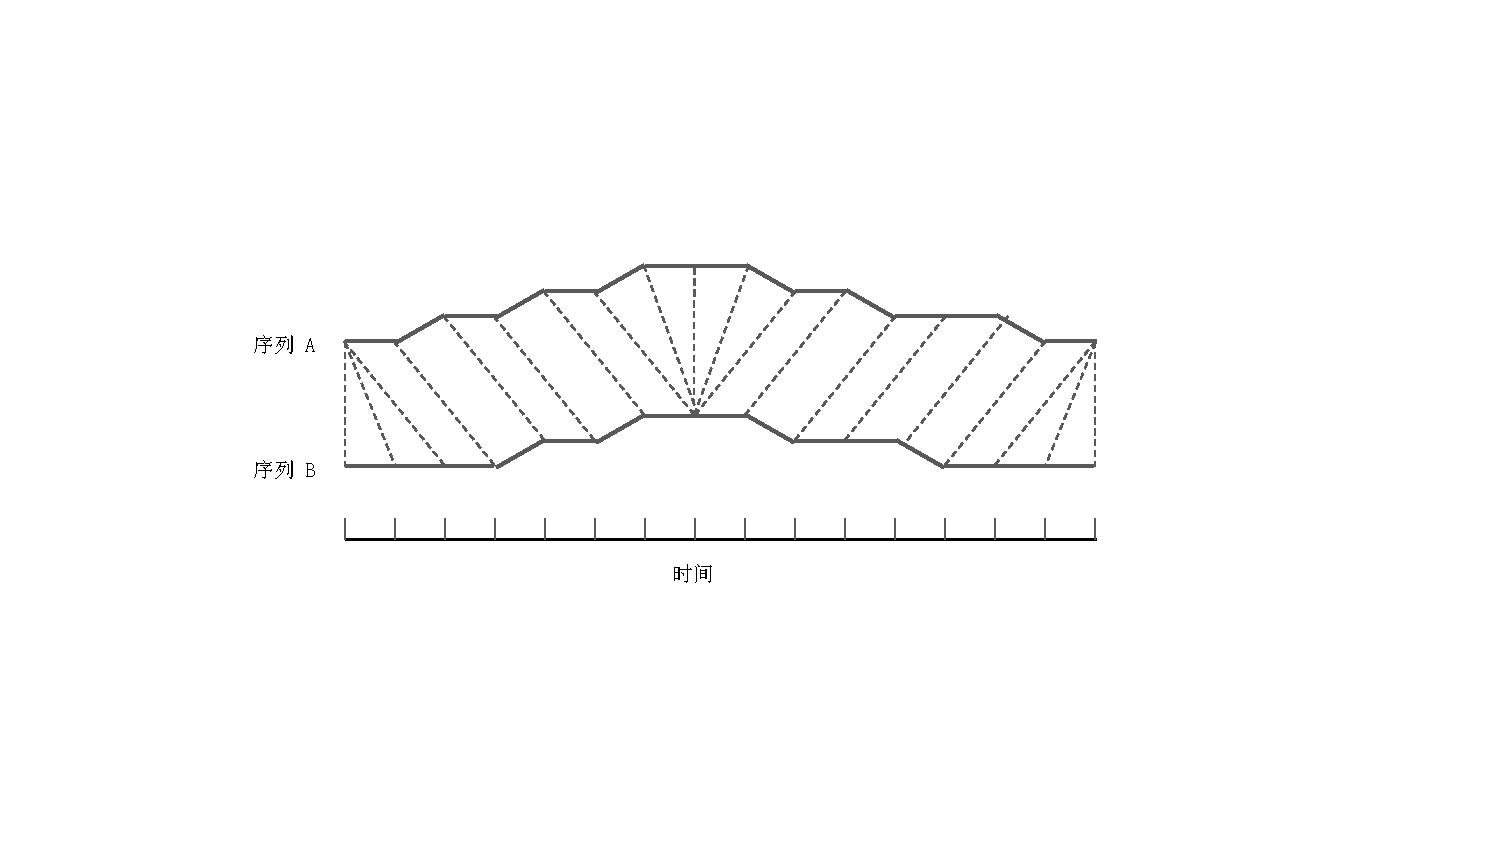
\includegraphics[width=13cm,trim=100 120 150 110,clip]{figure/2_dtw.pdf}
    \bicaption[DTW算法序列对齐示意图]
    {DTW算法序列对齐示意图}
    {Schematic diagram of DTW alignment algorithm}
    \label{fig:dtw}
\end{figure}

对于长度不一致的问题,比较容易想到的方法是通过拉伸的方法将较短的音频拉长到与较长音频长度相同,但是两段语音之间
的长度差距并不是等比例的,即对于内容中的一些字词,原始说话人说的较快,而对于另外一些字词,目标说话人则说的较快。
等比例的拉伸并不能做到较好的帧级别对应。
除此之外,最常用的特征对齐方法就是动态时间规整(Dynamic Time Warpingm, DTW)算法。该算法通过动态规划
来计算两个特征序列之间的最短距离,同时保存该最短距离所对应的路径。如图~\ref{fig:dtw}所示,上下两条粗线为两个特征序列,
中间的虚线代表特征的一一对应关系,对应关系的序列就是两个序列的最短路径。DTW通过计算两个序列之间的最短路径来实现对齐。
然而DTW算法仍有较大的对齐误差,尤其是对于差别较大的特征片段,而较大的对齐误差对转换效果的影响非常大。
因此研究人员将更多的注意力放在了无需对齐的方法上。非平行语音转换方法大多不需要对齐操作,这也是其优势之一。

\section{声学特征转换方法}
声学特征转换是语音转换中最重要的部分,也是当前主要的研究对象。声学特征的转换通常需要一个转换模型来完成,转换模型输入
原始声学特征序列,输出转换后的目标声学特征。本节主要介绍平行语料下的特征转换方法,非平行语料下的特征转换方法将在下一章
中详细介绍。

\subsection{混合高斯模型法}
混合高斯模型法是在深度学习方法之前使用最为广泛的方法之一。该方法使用混合高斯模型(Gaussian Mixture Model, GMM)
对原始说话人声学特征建模,并通过转换函数将原始特征转为对应的目标特征。设原始特征向量为$\mathbf{x}$,用GMM模型表示
其概率分布为
\begin{equation}
    \label{eq:gmm}
    p(\mathbf{x})=\sum^{m}_{i=1}\alpha_iN(\mathbf{x};\bm{\mu}_i,\bm{\Sigma}_i)
\end{equation}

其中$N(\mathbf{x};\bm{\mu},\bm{\Sigma})$代表均值为$\bm{\mu}$,协方差矩阵为$\bm{\Sigma}$的$p$维高斯分布,
可以表示为

\begin{equation}
    N(\mathbf{x};\bm{\mu},\bm{\Sigma})=\frac{1}{(2\pi)^{p/2}}\left| \bm{\Sigma} \right|^{-1/2} exp\left[ -\frac{1}{2}(\mathbf{x}-\bm{\mu})^{T}\bm{\Sigma}^{-1}(\mathbf{x}-\bm{\mu}) \right]
\end{equation}

公式中$\alpha_i$是归一化的正标量权重($\sum^{m}_{i=1}\alpha_i=1$ and $\alpha_i \ge 0$)。在GMM的语音转换
方法中,一个基本假设是声学特征的向量之间是相互独立的,即$t$时刻的目标特征向量$\mathbf{y}_t$只依赖与同一时刻的原始特征
向量$\mathbf{x}_t$。而GMM的一个优点是可以在不同的分布分量中进行软分类,在某种程度上,每一个类别可以代表不同的音素,或其他
音素相关的声学分类。给定观测向量$\mathbf{x}$,判断其属于GMM中一个声学类别$\mathcal{C}_i$的条件概率可以表示为

\begin{equation}
    P(\mathcal{C}_i|\mathbf{x})=\frac{\alpha_iN(\mathbf{x};\bm{\mu}_i,\bm{\Sigma}_i)}{\sum^m_{j=1}N(\mathbf{x};\bm{\mu}_j,\bm{\Sigma}_j)}
\end{equation}

GMM的参数可以通过期望最大化(Expectation-Maximization, EM)算法来估计。用GMM模型在原始声学特征上建模后,
则需要一个转换函数来将输入的原始特征向量转变为对应的目标特征向量,可以定义转换函数如下

\begin{equation}
    \mathcal{F}(\mathbf{x}_t) = \sum^m_{i=1}P(\mathcal{C}_i|\mathbf{x}_t)\left[ \mathbf{v}_i + \bm{\Gamma}_i \bm{\Sigma}_i^{-1} (\mathbf{x}_t-\bm{\mu}_i) \right]
\end{equation}

转换函数的参数只要是$\mathbf{v}_i$和$\bm{\Gamma}_i$,输入其中$\mathbf{v}_i$表示目标特征的期望均值,$\bm{\Gamma}_i$表示原始特征与目标特征的协方差矩阵。
这些参数通过最小化转换的均方误差来估计。误差可表示为

\begin{equation}
    \epsilon = \sum^n_{t=1} \left| \left| \mathbf{y}_t - \mathcal{F}(\mathbf{x}_t) \right| \right|^2
\end{equation}

该方法可以通过只对原始特征进行GMM建模来实现逐帧的语音转换。在此之后,一些基于GMM对目标特征建模的方法也被提出\cite{kain1998spectral}。
但是混合高斯法建立在不同帧之间相互独立的假设之上,只能实现逐帧转换,这是限制GMM转换性能的一个主要因素。

\subsection{码本映射法}
码本映射法(Codebook Mapping)的历史比混合高斯法更为悠久,是最早出现的语音转换方法之一。直观的码本映射法即是将原始和目标特征合并在一起,
训练一个大的码本。在转换时,原始特征先通过码本得到码本编号,与该编号最接近的目标特征即是转换特征。之后研究人员在码本映射法中加入了矢量量化(Vector Quantization, VQ)
的方法。该方法先对原始和目标特征通过VQ各自生成一个码本。同时对平行特征序列用DTW算法进行对齐,根据特征之间的对应关系生成直方图。对于原始说话人
每个码本向量的直方图,通过加权平均得到该码本向量对应的码本映射。在转换阶段,对原始特征的每一个特征向量,先通过原始说话人的码本编码得到量化向量,
再用该向量对应的码本映射得到转换特征。

码本映射法的基本思想简单直接,但也有比较明显的缺陷。首先逐帧转换对转换语音的连贯性有很大的影响,其次对声学特征离散化表示进行聚类会损失较多的声学信息,导致转换单一,自然度较差,
以及线性平均造成的严重过平滑问题。
对于这些缺陷,研究人员也提出一些改进措施比如码本词的线性加权组合法、分层的码本映射法和局部线性转换法等等。

\subsection{频率弯折法}
频率弯折法与之前介绍的语音转换方法不同,它是基于规则的语音转换方法。频率弯折法一般是通过频域中较为突出的区域特征来建立
原始与目标的映射关系(如共振峰的中心频率)。比较典型的频率弯折法是基于声道长度归一化(Vocal Tract Length Normalization, VTLN)的语音转换方法。

在基于VTLN的方法中,最优频率弯折函数$\mathcal{w}(\mathcal{f}, \theta)$的参数可以定义为

\begin{equation}
    \theta = \mathop{\arg\min}_{\theta}\int^{\pi}_{\mathcal{w}=0}\left| Y(\mathcal{f})-X(\mathcal{w}(\mathcal{f},\theta)) \right|^2 d\mathcal{w}
\end{equation}

其中$X(\mathcal{f})$和$Y(\mathcal{f})$分别代表原始和目标频谱。一般频谱弯折函数中只有一个参数$\theta$,
常见的弯折函数有二次函数

\begin{equation}
    \mathcal{w}_{\theta}(\mathcal{f}) = \mathcal{f} + \theta\left[ \frac{\mathcal{f}}{\pi}-(\frac{\mathcal{w}}{\pi})^2 \right]  
\end{equation}

以及双线性函数

\begin{equation}
    \mathcal{w}_{\theta}(\mathcal{f}) = \frac{\mathcal{f}-\alpha}{1-\alpha \mathcal{f}}
\end{equation}

频率弯折法通过对频谱中最显著的部分进行连续函数变换来实现语音转换,这样做的好处是可以在保留频谱中的大部分信息的前提下,
保证频谱的连贯性。因此频率弯折法往往可以得到比较好的音质,但是由于频谱中的说话人信息并不只包含在最显著的特征中,同时也存在于其他特征上(如共振峰带宽)。
因此频率弯折法的主要缺陷在于转换音频的说话人相似度较低。

\subsection{神经网络法}
神经网络(Neural Networks, NN)是一种从生物学中受到启发的建模方式。神经网络的发展历史较早,但早期多专注于理论阶段和复杂度相对较小的模型实验,
因此也提出了很多模型结构但难以验证。
随着大数据和计算机硬件的飞速发展,神经网络模型的参数量可以随着训练数据量的增多和计算速度的变快而不断地增加,从而可以实现更为复杂的
网络结构和建模任务,我们称之为深度学习。由于神经网络具有强大的建模能力,使得其在很多建模任务上相较传统的机器学习算法都取得了突破性的进展。如今,神经网络
已经在很多领域得到了广泛的应用,如计算机视觉,自然语言处理和智能语音等。

\begin{figure}[!htp]
    \centering
    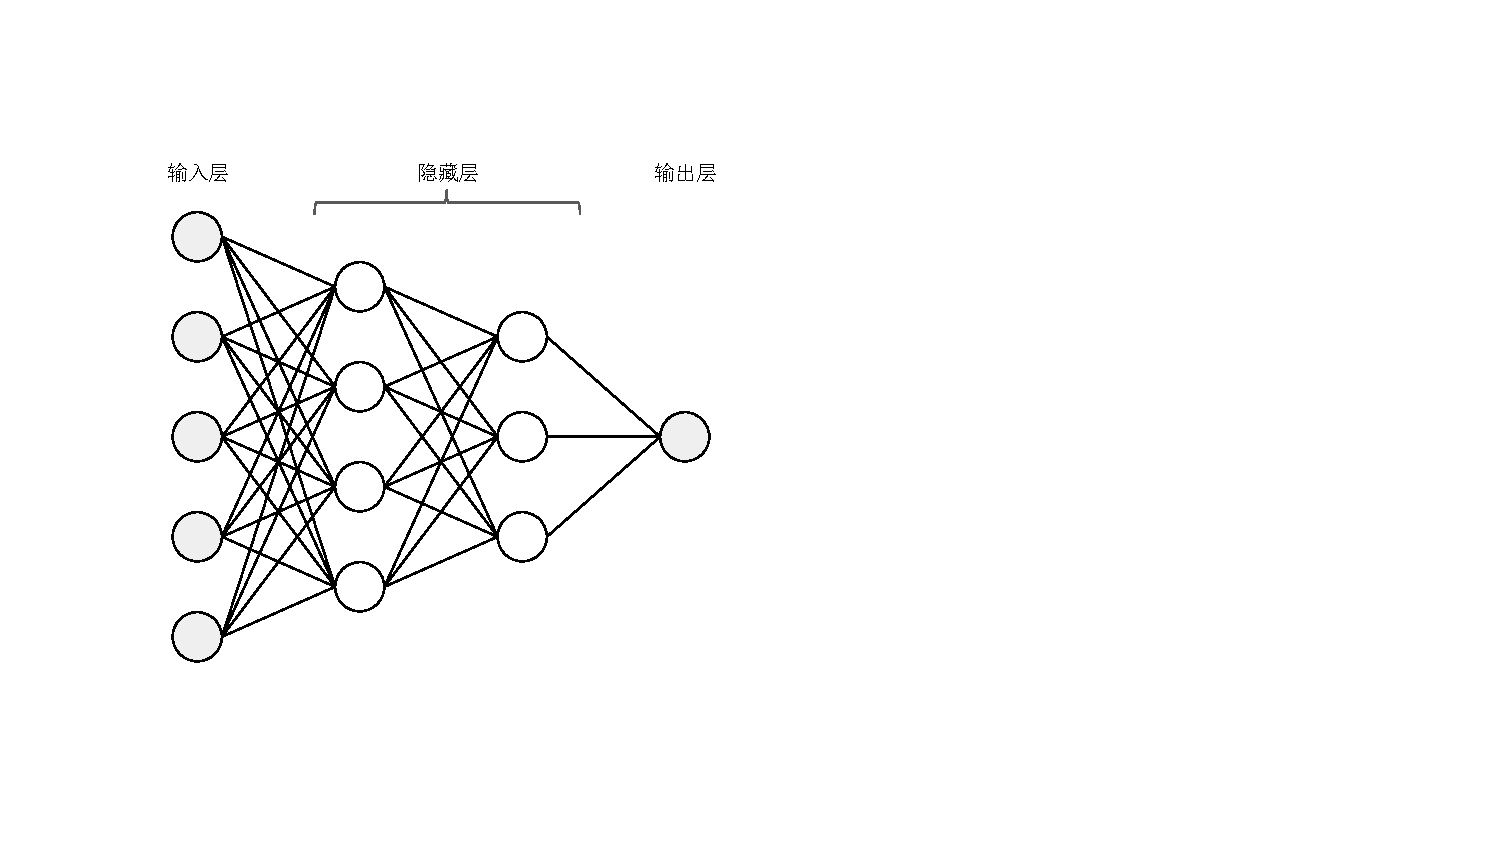
\includegraphics[width=8cm,trim=50 80 330 60,clip]{figure/2_mlp.pdf}
    \bicaption[多层感知机结构图]
    {多层感知机结构图}
    {Architecture of the Multilayer Perceptrons}
    \label{fig:mlp}
\end{figure}

最初的神经网络由多层感知机发展而来(Multi-Layer Perceptrons, MLP)。如图~\ref{fig:mlp},MLP由一个输入层,多个隐藏层,一个输出层组成。每一层都
包含有多个神经元,每个神经元都可以对输入做加权线性变换,并将结果输出。经过逐层的前向传播,MLP在输出层输出模型结果。在训练时,
MLP的输出会根据对应的标签计算误差,并使用反向传播(Back Propagation, BP)算法计算梯度,并根据每个参数的梯度更新模型。
从而使得模型可以不断的拟合训练数据。在数据量较大的情况下,神经网络具有较强的泛化能力,在测试集上的性能往往要好于传统方法。
在深度学习时代,神经网络的种类层出不穷,其中较为著名的包括深度神经网络(Deep Neural Networks, DNN),循环神经网络(Recurrent Neural Networks, RNN),
卷积神经网络(Convolutional Neural Network, CNN)等,其中每个网络也有较多的变种。

基于人工神经网络(Artificial Neural Networks, ANN)的语音转换方法在2009年被提出\cite{desai2009voice}。
作者用4层的神经网络学习原始特征到目标特征的映射关系,相邻两层之间采用全连接的形式。
在训练阶段,首先从原始和目标音频中分析,25维的梅尔倒谱系数和1维基频特征;然后用DTW算法对平行特征序列进行对齐,模型的输入是原始特征,标签是目标特征;
最后使用反向传播算法对模型进行训练。论文中的实验结果说明了基于神经网络的语音转换方法在主观实验和客观实验上都普遍好于基于GMM模型的语音转换方法。
该工作证实了神经网络在语音转换任务上的可行性。之后针对类ANN网络的语音转换改进方法也不断被提出。

\begin{figure}[!htp]
    \centering
    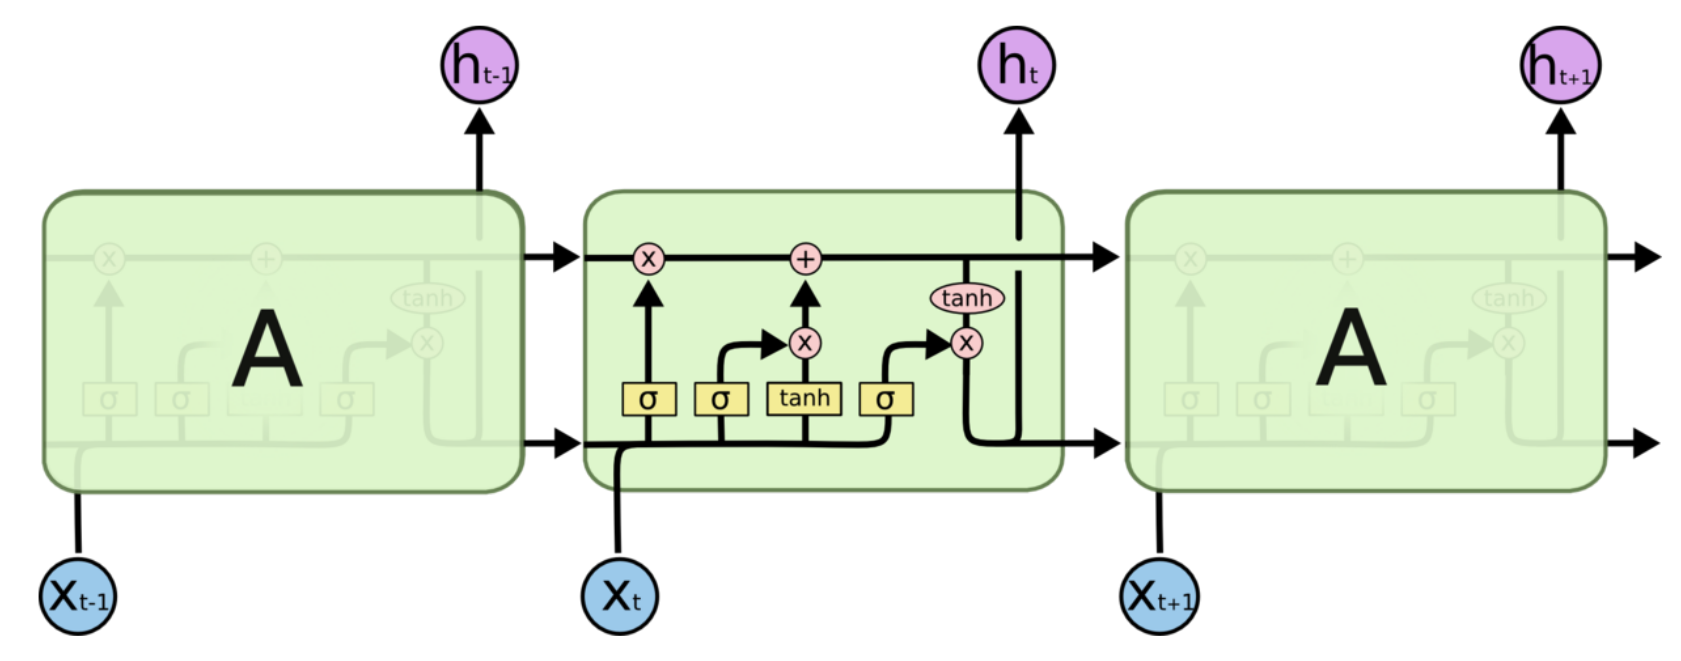
\includegraphics[width=10cm,trim=0 0 0 0,clip]{figure/lstm.png}
    \bicaption[长短时记忆网络结构图]
    {长短时记忆网络结构图}
    {Architecture of the Long Short Term Memory}
    \label{fig:lstm}
\end{figure}

如前文所述,很多方法都存在声学特征帧相互独立的假设,然而这个假设与常识有所矛盾,语音作为一个时序序列,距离越近的时刻往往相关性就越大。即使有些方法
也被提出来弥补这方面的缺陷,如加入动态特征,当前方法仍然没有很好的贴合时间序列的特性来实现更好的转换性能。在2015年,研究人员提出了基于
深度双向长短时记忆网络(Deep Bidirectional Long Short Term memory, DBLSTM)的语音转换方法\cite{sun2015voice}。该方法创新点主要为使用了包含DNN和双向LSTM的
转换模型。LSTM是RNN的一个变种,针对RNN对长时信息的建模能力较差,LSTM在RNN的单元(cell)中加入了三个门控机制,分别为输入门,遗忘门和输出门。
单元的状态值代表历史时刻的信息,其在网络的序列计算中不断更新。
如图~\ref{fig:lstm}所示,三个门控会通过$sigmoid$函数输出0到1之间的值,输入门表示当前时刻输入加入单元状态值的比例,
遗忘门表示当前时刻要从单元状态值中遗忘多少信息,输出门表示从更新后的单元状态值中输出多少比例到下一单元。设输入特征序列
$\mathbf{x}=\left\{x_1,x_2,...,x_T\right\}$,当前隐藏层的激活值为$\mathbf{h}=\left\{h_1,h_2,...,h_T\right\}$,
LSTM单元在$t$时刻的计算过程可以用如下公式表示

\begin{align}
    & i_t = \sigma (W_{i}x_t + U_ih_{t-1}+b_i) \\
    & f_t = \sigma (W_{f}x_t + U_fh_{t-1}+b_f) \\
    & c_t = f_tc_{t-1} + i_ttanh(W_cx_t+U_ch_{t-1}+b_c) \\
    & o_t = \sigma (W_{o}x_t + U_oh_{t-1}+b_o) \\
    & h_t = o_ttanh(c_t)
\end{align}
  
其中$\sigma$表示$sigmoid$激活函数,$W$和$U$为可学习的矩阵参数,$i$,$f$和$o$分别代表输入门,
遗忘门和输出门,$c$表示单元状态。双向网络在单向网络的基础上添加了额外一层,该层以由后向前的时间顺序
传播,两个相反方向的LSTM层输入同一个特征序列,并将输出的隐层序列拼接起来,形成最终的输出。在\cite{sun2015voice}中,
转换模型由6层BLSTM网络组成,并使用基于时间的反向传播算法(Back-Propagation Through Time, BPTT)训练模型。实验表明,
基于DBLSTM的转换模型明显好于基于DNN的方法。对比加入动态特征的DNN方法,DBLSTM模型在平均意见分(Mean Opinion Score, MOS)上
高出0.5分。

上面所述方法都有效促进了语音转换音质的提升,但这些方法都会受到特征对齐准确度的限制。如前文所述,特征对齐的准确度对语音转换有
很大的影响,目前所用到的特征对齐方法普遍还是基于DTW算法,而韵律差别较大的特征序列往往会使DTW算法的准确度急剧下降。
因此,基于序列到序列和注意力机制(Sequence-to-Sequence Attention)的语音转换模型于2019年提出\cite{tanaka2019atts2s}。序列到序列和注意力机制
模型是序列建模中非常著名的模型,它可以实现不受输入长度约束的不定长输出。序列到序列和注意力机制模型通常由三个模块构成:编码器,
注意力模块和解码器。其中编码器对输入的特征序列进行变换,将其转换成相同长度的抽象特征序列;解码器采用自回归的计算方式,输入
上一时刻的输出,和当前时刻注意力机制计算的注意力向量进行拼接,再去预测当前时刻的输出;注意力机制是一种序列相似度的对齐机制,
其输出向量的物理意义是指与当前解码器输入向量(Query, Q)最相似的编码器输入向量(Key, K)的特征值信息(Value, V)。公式表示如下

\begin{equation}
    \mathbf{c}_t = \sum^n_{i=1}\alpha_{t, i}\mathbf{h}_i
\end{equation}

其中$\alpha_{t, i}$表示$t$时刻输入与第$i$个编码器输入向量的匹配程度。$\mathbf{h}_i$代表第$i$个输入向量。
$\alpha$的计算方法如下

\begin{equation}
    \alpha_{t, i} = \frac{exp(score(\mathbf{s}_{t-1},\mathbf{h}_i))}{\sum^{n}_{i^{'}=1}exp(score(\mathbf{s}_{t-1},\mathbf{h}_{i^{'}}))}
\end{equation}

$\mathbf{s}$是指编码器输入向量。$score$的计算方法有很多种,如余弦法,点乘法,基于位置的方法等。
注意力机制在解码器解码时向其提供输入序列的局部信息,以使解码结果与输入的对应位置保持一直,另一方面,
注意力机制可以完成更为复杂的对齐操作,可以实现相比DTW更为准确的对齐路径,从而提升转换性能。除此之外,
论文中也额外添加了一个编码器和一个解码器,通过对原始特征序列和目标特征序列进行重构,来尽可能在转换过程中
保留特征中的语义信息。实验证明,该方法的转换语音在自然度和相似度上都要好于基于GMM的语音转换方法,
另外该方法也好于基于LSTM的语音合成方法。这也是目前在平行语音转换任务上转换音质最好的方法之一。

\section{韵律转换}
韵律一般是指语音的发音节奏,语速和表现力等,与说话人的说话风格有很大的关系,准确的韵律转换可以使
转换语音更接近目标说话人。与韵律相关的特征主要有基频和时长,下面将对这两种特征的主要转换方法做以说明。

\subsection{基频转换}
基频(Fundamental Frequency, F0)代表着语音当中的最低频率,由于基频在人耳的感知中具有最大的响度,
因此基频常与语音的音调等价。基频的转换是十分必要的,尤其对于跨性别语音转换,男性的基频分布与女性的
基频分布往往差别较大,此时基频的转换效果会直接影响转换语音的相似度。

传统的基频转换方法通常使用均值方差归一化的线性转换。该方法非常简单直接,首先从原始和目标训练数据中提取基频序列;
然后分别计算原始基频序列和目标基频序列的均值($\mu_s$, $\mu_t$)和方差($\sigma_s$,$\sigma_t$);在转换阶段,对原始测试基频用原始说话人的均值方差先做归一化,
再用目标说话人的方差均值对其做逆归一化。转换过程可用公式表示如下

\begin{equation}
    F_0^t = (F_0^s - \mu_s)\frac{\sigma_t}{\sigma_s} + \mu_t
\end{equation}

其中$F_0^s$和$F_0^t$分别代表原始基频和转换目标基频。在乐理中,基频在对数域会呈现等差增长,
即音高频率在对数域是平均分布的,且在\cite{erro2009voice}中,基频在对数域比在
线性域能够更好地被正态分布拟合。因此在实际操作中更倾向于以对数基频为线性转换的对象。

然而线性变换也存在明显的缺陷,该方法只能改变基频的分布,而不能改变基频的变化趋势。在\cite{chen2018high}中,
作者在平行语料的语音转换任务中,使用梅尔频谱特征代替传统的数字信号声码器分析特征(梅尔倒谱系数,基频,非周期成分),
直接用转换模型学习梅尔频谱中基频信息的转换。经过实验验证,使用模型学习基频的隐式转换可以获得更接近目标基频轨迹的
转换语音。

\subsection{时长转换}
时长转换的常用方法与基频转换类似,也是使用线性转换的方法改变语速,即对一整句话进行固定比例的拉伸操作来改变时长,如线性插值或样条插值。
除此之外一些基于音素的韵律转换方法也被提出\cite{helander2007novel}。如前文所述,
在\cite{tanaka2019atts2s}中,序列到序列的建模方式可以有效实现不等长序列的映射关系学习,
同时也可以做到不定长序列的生成,该模型的解码器通过在每个时间步判断停止令牌(stop token)来决定
是否需要停止解码。但是,时长转换由于评价指标较难定义,且对说话人相似度的影响较小,目前研究的主要重心仍集中在
频谱转换上。

\section{本章小结} 
本章主要介绍语音转换系统的典型框架及其主要部分,包括语音分析和合成方法,
特征对齐,频谱转换方法和韵律转换方法。本章首先对语音转换系统,评价指标及常用特征进行了回顾;
然后介绍了语音转换系统中每个部分的主流技术及最新进展,并对其优势和不足进行了分析。作为语音转换中
最重要的部分,本文对常见的几种平行语料的频谱转换方法进行了详细的介绍。